\bookchapter{Bab 37: Revolusi paradigma - daripada “menulis kod” kepada “mengarah AI menulis kod”}

\chapterintro{Tahniah, anda yang membuka buku ini sedang berdiri di tengah-tengah revolusi paradigma kerjaya. Titik permulaan revolusi ini ialah satu ayat yang dihantar seorang pengaturcara di media sosial pada tahun 2025. Kedengaran agak dramatik? Tetapi itulah hakikatnya.}

\booksection{Kelahiran Vibe Coding: gerakan yang dicetuskan oleh satu ayat}

Pada Februari 2025, Andrej Karpathy - sila ingat nama ini dahulu, anda akan berjumpa dia beberapa kali lagi kemudian - menghantar satu twit yang kemudiannya banyak kali dipetik di media sosial: “Ada cara pengaturcaraan baharu yang dipanggil Vibe Coding, anda bergantung sepenuhnya pada perasaan (vibes), abaikan butiran kod, biarkan AI menguruskan segalanya. Apa yang anda nampak itulah yang anda katakan, salin dan tampal, asalkan boleh berfungsi.”

Ucapan yang kelihatan dibilang sambil lewa ini sebenarnya menamakan dengan tepat satu anjakan paradigma yang telah berlaku secara senyap: manusia tidak lagi menulis kod baris demi baris, sebaliknya menggambarkan niat dengan bahasa semula jadi, dan AI yang menyiapkan pelaksanaannya. Pilihan kata Karpathy membawa sedikit nada bergurau, tetapi di sebaliknya terdapat pemerhatian yang mendalam: apabila keupayaan penjanaan kod AI melepasi satu ambang tertentu, kepincangan pengaturcaraan bukan lagi “bolehkah saya menulis baris kod ini”, tetapi “adakah saya benar-benar memikirkan perkara ini dengan jelas”.

\begin{tcbinfo}{Tip: Apa itu Vibe?}
Vibe secara harfiah bermaksud “suasana, perasaan”. Vibe Coding ialah “mengarah AI mengatur cara mengikut perasaan” - anda menerangkan apa yang anda mahu, AI yang melaksanakannya. Ingat perkataan ini; ia ialah “sijil kelahiran” revolusi ini.

\end{tcbinfo}

Dari saat itu, maksud perkataan “pengekodan” mula terbelah: pengekodan tradisional menterjemahkan reka bentuk kepada sintaks; pengekodan baharu menterjemahkan niat kepada arahan. Yang pertama menguji jari, yang kedua menguji otak.

Perkataan Vibe Coding dengan cepat bertukar daripada gurauan kepada konsep kejuruteraan yang serius. Menjelang pertengahan 2026, ia telah berevolusi daripada satu jenaka di media sosial kepada satu sistem metodologi lengkap - merangkumi keseluruhan proses daripada penyataan keperluan, pengurusan konteks, pengesahan iteratif hingga jaminan kualiti. Orang juga sedar: “ikut perasaan” hanyalah keadaan peringkat permulaan; pengaturcaraan AI yang benar-benar cekap memerlukan cara berfikir yang tersusun. Dan cara berfikir inilah yang buku ini hendak berikan kepada anda.

\booksection{Keadaan 2026: era Agentic Engineering}

Menjelang Ogos 2026, bidang pengaturcaraan AI telah melalui beberapa iterasi paradigma yang penting. Vibe Coding ialah percikan awal, tetapi dengan cepat semua orang mendapati: berbual dengan AI hanya “ikut perasaan” menghasilkan kod yang kualitinya sangat tidak stabil - kadangkala mengagumkan, kadangkala gagal teruk. Maka paradigma mula berevolusi: daripada pengaturcaraan perbualan yang mudah kepada kejuruteraan Agent yang berstruktur.

Sekali lagi Karpathy, pada awal 2026 memperkenalkan konsep Agentic Engineering. Berbeza dengan “sebut sahaja, terus terjana” ala Vibe Coding, Agentic Engineering menekankan: beri AI satu matlamat, biarkan ia merancang langkah dengan sendirinya, menggunakan alat, mengesahkan hasil, dan membaiki secara beriterasi. AI bukan lagi sekadar penjana kod, tetapi satu ejen pintar (Agent) yang boleh merasai persekitaran, membuat keputusan, dan melaksanakan tindakan.

Peralihan ini membawa tiga perubahan utama:

\begin{enumerate}
  \item Mod interaksi berubah: daripada "satu soalan satu jawapan" kepada "tetapkan matlamat, kemudian beri kuasa".
  \item Hasil kerja berubah: daripada "sepotong kod" kepada "satu projek yang lengkap".
  \item Peranan manusia berubah: daripada "menyemak kod baris demi baris" kepada "menentukan sempadan dan menerima hasil".
\end{enumerate}

Angka tidak berbohong: dalam versi Cursor 3 yang dikeluarkan pada April 2026, kadar penggunaan mod Agent buat kali pertama mengatasi mod pelengkap Tab, menandakan pembangun sudah berpindah secara besar-besaran kepada cara kerja ini; manakala Claude Code, alat pengaturcaraan AI natif terminal, menjelang pertengahan 2026 telah mencapai saiz pendapatan tahunan sebanyak 2.5 bilion dolar AS. Carta arah aliran berikut membolehkan anda merasai secara langsung persilangan masa ini:

\begin{center}
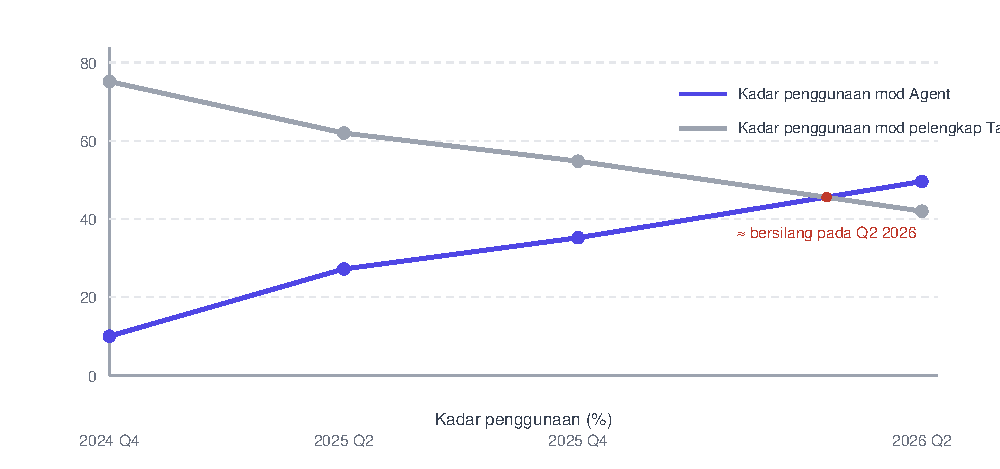
\includegraphics[width=0.92\linewidth]{figures/fig-di-san-shi-qi-zhang-1}
\\[2pt]\small Rajah 1: Trend perubahan kadar penggunaan mod interaksi pengaturcaraan AI (anggaran berdasarkan data kaji selidik industri; suku kedua 2026 mod Agent mengatasi pelengkap Tab)
\end{center}

Tetapi secara jujur: perubahan alat dan model hanyalah yang kelihatan di permukaan. Sama ada anda guna Cursor atau Claude Code, sama ada model asasnya GPT-5 atau Claude 4.5, pengamal pengaturcaraan AI yang berjaya semuanya mengikuti satu metodologi asas yang sama. Inilah yang panduan ini hendak ajarkan kepada anda.

\booksection{Peralihan pemahaman teras: daripada Coder kepada Conductor}

Pendidikan pengaturcaraan tradisional mengajar anda bagaimana menjadi seorang Coder - memahami sintaks, menghafal API, menyahpepijat ralat logik. Pada era pengaturcaraan AI, peranan ini sedang ditakrifkan semula. Anda tidak lagi perlu menulis setiap baris kod dengan tangan sendiri, tetapi anda perlu menjadi seorang “konduktor” (Conductor): menentukan medan perang, membuat peraturan, membahagikan tugas, dan menerima hasil.

Teras peralihan ini bukan pada “bolehkah anda menulis kod”, tetapi pada “bolehkah anda memikirkan dengan jelas apa yang hendak dibuat”. Seorang konduktor yang cemerlang belum tentu tentera yang terbaik, tetapi dia paling jelas tentang matlamat pertempuran, rupa bumi, dan penempatan tentera. Begitu juga, pengamal pengaturcaraan AI yang cemerlang belum tentu menguasai butiran sintaks setiap bahasa pengaturcaraan, tetapi dia paling jelas tentang matlamat projek, kekangan seni bina, dan piawaian kualiti.

Jadual ini patut anda lihat lebih sekali - ia meringkaskan keseluruhan intipati peralihan peranan ini:

\begin{center}
\begin{tabularx}{\linewidth}{|X|X|X|}
\hline
\textbf{Dimensi} & \textbf{Coder tradisional} & \textbf{Konduktor AI (Conductor)} \tabularnewline
\hline
Kemahiran teras & Menghafal sintaks, memanggil API, menyahpepijat & Takrif keperluan, pengurusan konteks, pertimbangan penerimaan hasil \tabularnewline
Cara kerja & Menulis kod baris demi baris & Menerangkan niat, menyemak hasil \tabularnewline
Kawalan kualiti & Yang ditulis sendiri, sendiri tahu kekuatan-kelemahannya & Mengesahkan hasil AI melalui ujian dan semakan \tabularnewline
Keperluan pengetahuan & Menguasai secara mendalam bahasa/rangka kerja tertentu & Memahami secara meluas gambaran teknologi keseluruhan, memahami secara mendalam logik perniagaan \tabularnewline
Letaknya kepincangan & Kelajuan pengekodan dan ingatan sintaks & Kejelasan berfikir dan keupayaan menyatakan \tabularnewline
Sumber ralat & Ralat sintaks, logik tertinggal & Keperluan kabur, konteks tidak cukup \tabularnewline
\hline
\end{tabularx}
\end{center}

\begin{center}\small\color{gray}Perbandingan dimensi kebolehan antara Coder tradisional dan Konduktor AI\end{center}

Ini sama sekali bukan bermakna pengetahuan pengaturcaraan tidak penting lagi. Sebaliknya: apabila anda dapat memahami kod yang ditulis AI, barulah anda boleh menyemak dan membaikinya dengan berkesan; apabila anda memahami struktur data dan algoritma, barulah anda dapat menilai sama ada penyelesaian AI munasabah. Simpanan pengetahuan menentukan “had pengarahan” anda - tetapi peranan pengetahuan bertukar daripada “alat pelaksanaan” kepada “asas pertimbangan”.

\booksection{Mengapa metodologi lebih penting daripada alat}

Alat berulang setiap tiga bulan, metodologi berevolusi setiap tiga tahun. Menguasai cara guna satu alat mungkin lapuk dalam tiga bulan; menguasai satu cara berfikir masih releven tiga tahun kemudian.

Banyak orang apabila mula belajar pengaturcaraan AI, perkara pertama yang ditanya ialah “alat mana paling bagus” “model mana paling kuat”. Soalan-soalan ini bukannya tidak penting, tetapi ia bertanya dengan keutamaan yang salah. Landskap alat pada Ogos 2026 sudah sama sekali berbeza daripada Ogos 2025 - alat seperti Trae dan Qoder berganti naik turun, Cursor bertukar daripada plugin kepada IDE berdikari lalu berevolusi ke Cursor 3, Claude Code bertukar daripada projek eksperimen kepada pilihan utama pengaturcaraan terminal. Tetapi di sebalik perubahan hebat ini, prinsip pemikiran yang diikuti pengamal yang berjaya hampir tidak berubah.

Itulah sebabnya buku ini tidak akan menghabiskan halaman untuk mengajar operasi khusus sesuatu alat - kandungan sebegitu akan lapuk sebaik selesai ditulis. Sebaliknya, seluruh tumpuan buku ini diletakkan pada satu metodologi pemikiran yang telah terbukti: bagaimana memikirkan keperluan, bagaimana berkomunikasi dengan AI, bagaimana mengesahkan hasil, bagaimana mengiterasi secara berterusan. Dengan menguasai metodologi ini, anda boleh cepat mahir dengan apa-apa alat sekalipun ditukar; jika hanya belajar operasi alat, bertukar alat bermakna bermula dari sifar.

\begin{tcbinfo}{Penenang hati untuk pembaca sifar asas}
Jika anda sifar asas, jangan terkejut dengan perkataan “metodologi”. Metodologi bukan falsafah abstrak; ia sememangnya satu manual operasi “bagaimana untuk berfikir apabila menghadapi masalah”. Seperti belajar memasak: anda boleh ikut resipi langkah demi langkah (operasi alat), tetapi koki sebenar memahami “mengapa perasa begini” dan “bagaimana mengawal suhu api” (metodologi). Buku ini akan bermula daripada konsep paling asas, dan setiap prinsip disertakan dengan contoh perbandingan yang konkrit, memastikan anda bukan sahaja memahami “apa itu”, malah menguasai “bagaimana melakukannya”.

\end{tcbinfo}

\begin{tcbpractice}{Mari praktik: ambil "gambar peranan" untuk diri anda sekarang}
Ambil sekeping kertas, tulis jawapan untuk tiga soalan: (1) Bagaimana anda kini menggunakan AI untuk membantu menulis kod (jika pernah guna)? (2) Anda lebih serupa “Coder” atau “konduktor” dalam jadual di atas? (3) Bagaimana mungkin diri anda tiga bulan lagi akan menerangkan cara kerja anda? Selepas menulis, selitkan dalam buku ini, dan lihat semula selepas membaca Bab 47 - anda akan mendapati perubahan lebih cepat daripada jangkaan.

\end{tcbpractice}

\begin{tcbsummary}{Ringkasan bab ini}
\begin{itemize}
  \item Pada 2025 Karpathy menamakan revolusi pengaturcaraan AI dengan "Vibe Coding": daripada menulis kod baris demi baris kepada menerangkan niat dengan bahasa semula jadi
  \item Pada 2026 berevolusi kepada Agentic Engineering: beri matlamat, beri kuasa, AI merancang dan melaksanakan sendiri, manusia bertanggungjawab menerima hasil
  \item Kadar penggunaan mod Agent Cursor 3 buat kali pertama mengatasi pelengkap Tab; pendapatan tahunan Claude Code mencapai 2.5 bilion dolar AS
  \item Peranan baharu anda ialah Conductor (konduktor): menentukan medan perang, membuat peraturan, membahagikan tugas, menerima hasil
  \item Alat beriterasi setiap tiga bulan, metodologi hanya berevolusi setiap tiga tahun - pelajari metodologi, bukan operasi
\end{itemize}

\end{tcbsummary}
